\subsection{LLM-as-a-CoT-Judge for Math Reasoning}
\label{supp_sec:verify_details}

\begin{figure}[ht]
    \centering
    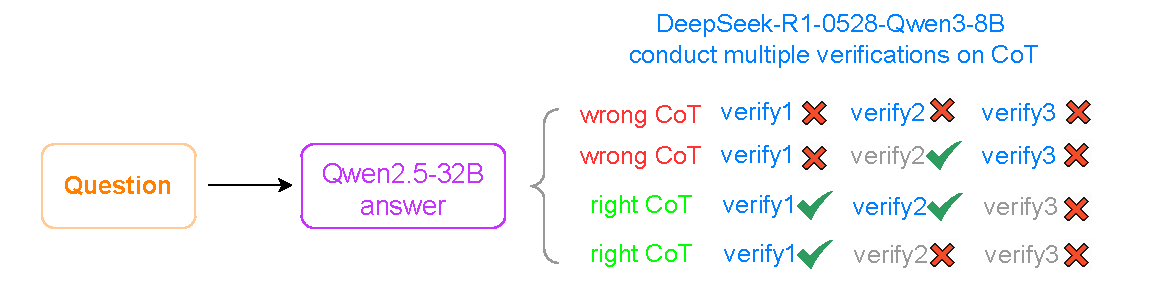
\includegraphics[height=10em]{figures/multi_verify.pdf}
    % \caption{Verification accuracy across multiple turns to ensure full recall}
    \caption{An intuitive diagram to illustrate the benefits of our multi-verification system: simultaneously considering \emph{any-correct}, \emph{all-correct}, and \emph{majority-correct} helps us to mitigate false positives and false negatives within individual verifications.}
    \label{fig:multi_verify}
\end{figure}

We use a much more specialized LLM on mathematical reasoning (DeepSeek-R1-0528-Qwen3-8B) as the verifier to examine the reasoning steps of base LLM, Qwen2.5-32B.
Meanwhile, we also acknowledge the existence of verification errors and manually checked many of them to confirm the reliability of this verification.
To further mitigate potential verification errors, we design a multi-verification approach, as shown in Figure~\ref{fig:multi_verify}). For each reasoning CoT, we conduct multiple verifications independently and calculate three aggregation metrics:

\begin{itemize}
    \item \emph{All-correct}: Chains of Thought that pass all verification attempts
    \item \emph{Majority-correct}: Chains of Thought that pass most verification attempts
    \item \emph{Any-correct}: Chains of Thought that pass at least one verification attempt (capturing potential error recovery cases)
\end{itemize}

This multi-verification approach can ensure us to have a comprehensive view of CoT correctness because the \emph{all-correct} strategy mitigates false positives and the \emph{any-correct} option reduces false negatives.
Let $p_{\text{fp}}$ and $p_{\text{fn}}$ represent the per-attempt false positive and false negative rates, respectively. For $n$ independent verification attempts, we observe:

\begin{itemize}
    \item \emph{All-correct}: The false positive rate decays exponentially as $p_{\text{fp}}^n$
    \item \emph{Any-correct}: The false negative rate decays exponentially as $p_{\text{fn}}^n$
\end{itemize}

In our study, we employ $n = 3$ verification attempts for each CoT.

Moreover, we provide the prompt template used for DeepSeek-R1-0528-Qwen3-8B as follows.

\tcbset{colback=gray!5, colframe=black!80, fonttitle=\bfseries}
\begin{tcolorbox}[title=Our Prompt Template for Verifier DeepSeek-R1-0528-Qwen3-8B]

You are an expert in mathematics and logical reasoning. Your task is to evaluate the correctness of a solution to a given math problem, with a **strong emphasis on the reasoning process**, not just the final answer.

Below is the **Problem** and the **Solution (Provided by another AI model)**:

---

**Problem**:

\{\{question\}\}

**Solution (Provided by another AI model)**:

\{\{solution\}\}

---

Please perform the following tasks:

1. **Analyze the solution step-by-step**, paying close attention to:
   - Computational accuracy
   - Logical consistency
   - Conceptual understanding
   - Whether the reasoning is valid and complete

2. **Identify any issues or errors in the reasoning**, even if the final answer is correct. Classify them into the following categories (if applicable):
   - **Calculation Error**: Mistakes in arithmetic, algebraic manipulation, or numerical computation.
   - **Logical Error**: Invalid reasoning, flawed logic, or incorrect inference.
   - **Conceptual Error**: Misunderstanding or misuse of mathematical concepts or definitions.
   - **Omission / Incompleteness**: Missing steps, incomplete justification, or not addressing all parts of the question.
   - **Other**: Any other type of error that does not fit into the above categories.

3. **Provide a final judgment** on whether the solution is logically sound and free of errors in reasoning.

Please format your response as follows:

---

**Issues Identified:**

- [Issue 1]: [Classification] - [Brief explanation]
- [Issue 2]: [Classification] - [Brief explanation]
- ...

Let's think step by step and output your final judgment within \textbackslash boxed\{\}

\textbackslash boxed\{yes\} or \textbackslash boxed\{no\}

\end{tcolorbox}

% , which effectively balances the detection of incorrect Chains of Thought while reliably identifying correct ones.

% To prevent verification errors, we manually validated the more challenging cases and found that the model may indeed make occasional mistakes during multiple verification attempts.(Figure~\ref{fig:multi_verify}) Therefore, our visualization presents three distinct curves: \emph{all-correct}: indicating CoT that pass all verify turns; \emph{majority-correct}: indicating CoT that pass major verify turns;
% \emph{any-correct}, indicating CoT that pass any one of verify turns;
% to account for potential error recovery cases. The challenge cases we study can be correctly classified by at least one of these metrics (ensuring full recall).

% We let $p_{\text{fp}}$ and $p_{\text{fn}}$ denote the per-attempt false positive (FP) and false negative (FN) rates. For $n$ independent verification attempts:

% \begin{itemize}
%     \item \textbf{Correct All}: FP rate $\rightarrow p_{\text{fp}}^n$ (exponential suppression)
%     \item \textbf{Correct Any}: FN rate $\rightarrow p_{\text{fn}}^n$ (exponential suppression)
% \end{itemize}

% In this study, we adopt $n = 3$ and find that this setup helps to detect incorrect CoTs and recognize correct ones.

% The multi-verification system guarantees:
% $$
% \lim_{n\to\infty} R_{\text{joint}} \leq \min(p_{\text{fp}}, p_{\text{fn}})
% $$
% with "Correct All" strictly bounding FP and "Correct Any" bounding FN.